%% ★★★★ §2 "Background" IS MERGED INTO §1 (sections/01_intro.tex).  Both
%% referees asked for it: "merge background into introduction", "§1-§2: merge
%% into one Introduction of about 1 page".  This file is kept, and keeps its
%% \input line, because it still carries Table 1 and Figure 1 -- the two
%% floats the merged introduction cites.  \label{sec:background} is RETIRED
%% and its three external references repointed at \label{sec:intro}
%% (04_method.tex, 06_discussion.tex, 07_conclusions.tex), because keeping two
%% labels on one anchor fails labelcheck's F7.
%%
%% The prose that was here and is now in 01_intro.tex, compressed: the
%% centimetre heritage (one paragraph, every citation key kept -- see below),
%% the empty record above 30 GHz, Steffes/Mauersberger, the Band 1 coverage,
%% the Mason comparison and the Figure 1 paragraph.
%%
%% DELETED OUTRIGHT, as instructed: the Arecibo planetary-radar EIRP sentence
%% ("the Arecibo planetary radar had an EIRP of \AreciboW W at \ArecGHz GHz;
%% an aperture of that diameter is not realisable in the millimetre band").
%% \AreciboW and \ArecGHz were cited nowhere else and retire with it.  The
%% CWTFM normalisation in §6.2 uses a DIFFERENT macro, \FomAreciboEirp, and is
%% untouched; make_fig_context_v410.py's assertion that no Arecibo-equivalent
%% line is drawn on any panel does not read either macro.
%%
%% ★ EVERY CITATION KEY IS KEPT.  citegate's G1 requires every \bibitem to be
%% cited, and all thirteen centimetre-survey keys have exactly ONE citation
%% site, so "reduce the centimetre programmes to representative references"
%% cannot shorten the reference list without deleting bibitems.  The prose is
%% what was long; a \citep list costs a few characters.  Dropped prose, kept
%% keys: the MWA correlator and Sardinia descriptions.

\begin{table}
\centering
%% ★ v4.26 (r25-captions): 4 printed lines -> the author's 3.  \S\ref{sec:intro}
%% already says this table "gives each programme's threshold, the factor that
%% puts it on the common basis and the channel width it used", so the clause
%% listing the columns was saying it twice.  The two column DEFINITIONS stay.
\caption{The comparison programmes of Figure~\ref{fig:context}
(\S\ref{sec:intro}). $\mathrm{EIRP}_{\rm min}$ is the deepest limit each
paper reports; the factor is $\LtCommonSnr/(\mathrm{S/N})$.}
\label{tab:litthresh}
\scriptsize
\setlength{\tabcolsep}{4pt}
%% GENERATED by make_fig_context_v410.py -- do not hand-edit.
\begin{tabular}{@{}lccccc@{}}
\toprule
programme & S/N & factor & $\Delta\nu_{\rm ch}$ & EIRP$_{\rm min}$ & at $5\sigma$ \\
 & & & & (W) & (W) \\
\midrule
Enriquez\,+\,17 & 25 & 0.20 & 2.8\,Hz & $5.2\times10^{12}$ & $1.04\times10^{12}$ \\
Margot\,+\,23 & 10 & 0.50 & 3.0\,Hz & $1.35\times10^{13}$ & $6.75\times10^{12}$ \\
Price\,+\,20 & 10 & 0.50 & 2.8\,Hz & $2.1\times10^{12}$ & $1.05\times10^{12}$ \\
Mason\,+\,25 & 5 & 1.00 & 30.5\,kHz & $6.91\times10^{17}$ & $6.91\times10^{17}$ \\
\bottomrule
\end{tabular}

\end{table}

%% ★ Table 1's caption was 6 printed lines.  Removed: "the minimum detectable
%% flux being linear in the threshold in every one of their own expressions
%% for it", which justifies the factor rather than defining it, and is the
%% kind of methodological explanation R1 asks to be taken out of captions.
%% The justification is not lost: it is the definition of the rescaling, and
%% §1 states that the rescaling puts thresholds on one arithmetic convention
%% and not at a matched false-alarm probability.

\begin{figure}
\centering
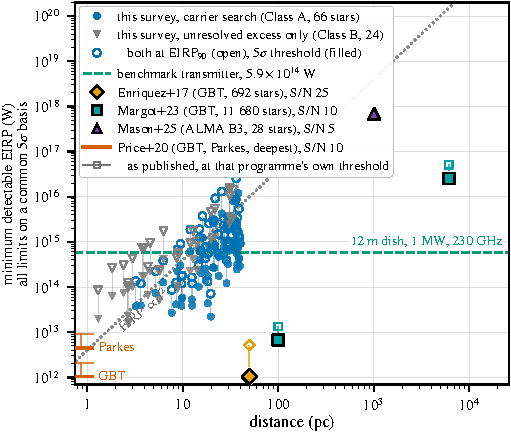
\includegraphics[width=\columnwidth]{figures/eirp_context_a.pdf}\\
{\footnotesize (a)}\\[4pt]
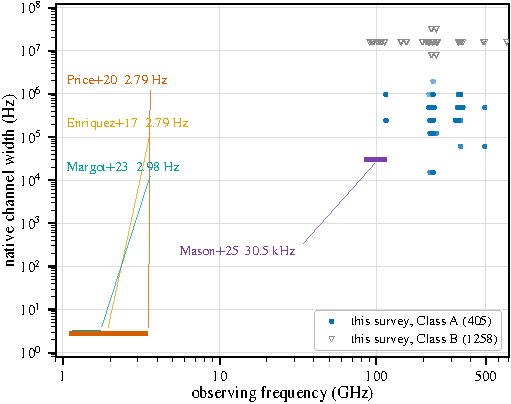
\includegraphics[width=\columnwidth]{figures/eirp_context_b.pdf}\\
{\footnotesize (b)}
%% ★★★ v4.26 (r25-captions): 16 PRINTED LINES -> R1 §7's limit of about six.
%% MOVED into \S\ref{sec:intro}, where Fig.~1 is discussed, and carrying with
%% it three macros THIS CAPTION WAS THE ONLY CITATION SITE OF -- \LtChanSpanDex,
%% \LtChanNarrow, \LtChanWide -- and a fourth, \NgNDecBOnly: the native-channel
%% span and what it means for comparing two programmes; "no limit plotted
%% carries a confirmation criterion"; the grey triangles constraining an
%% unresolved excess and not a carrier; and "the only symbols carrying
%% measured completeness".  Deleting instead of moving would have let
%% retire_macros.py take four numbers out of the paper in silence.
%% DELETED, because the drawn panels already carry it or \S1 already says it:
%% "each published value kept beside its rescaled one" (\S1 states exactly
%% that of the rescaling) and the list of what the panels label, which they
%% do label -- \BenchDiam keeps two citation sites elsewhere.
\caption{Where this survey sits among published radio technosignature
searches, on Table~\ref{tab:litthresh}'s common $\LtCommonSnr\sigma$ basis
(\S\ref{sec:intro}). \textbf{(a)} Minimum detectable EIRP against distance;
this survey's deepest window per star -- blue, the carrier search; grey,
coarse channels only; filled, the bare threshold; open,
$\mathrm{EIRP}_{90}$. \textbf{(b)} Native channel width against sky
frequency (filled, Class~A; open, Class~B).}
\label{fig:context}
\end{figure}

%% ★ Figure 1's caption was 30 printed lines, 1848 characters, the longest in
%% the main text; the referees asked for about 60 per cent off, and it is now
%% 17 printed lines / 1023 characters, measured by capmeasure.py.
%% WHAT WENT: the colour legend (orange/aqua/violet/left-edge ticks, grey
%% dotted, green dashed) -- "the panel labels already carry the legend", and
%% they do, the panels print Parkes, GBT, Price+20, Enriquez+17,
%% EIRP propto d^2 and "12 m dish, 1 MW, 230 GHz"; the sentence re-explaining
%% the rescaling; and the "Compare the hollow markers with this survey's
%% filled ones" aside.
%% WHAT STAYED, because each is a caveat and not an explanation: the native
%% channel span (a limit is only a limit for a signal narrower than the
%% channel that set it), the Class B triangles constraining an unresolved
%% excess and NOT a drifting carrier, completeness measured only for this
%% survey's open symbols, and no confirmation criterion anywhere on the
%% figure.  Two caveats MOVED into §1 so each survives exactly once: the
%% matched-false-alarm qualification, which §1 states where the rescaling is
%% described, and "excludes atmospheric decorrelation", which Table 3 defines
%% as the meaning of "nominal".
%% ► Enriquez2017 and Price2020 keep citation sites elsewhere, so dropping
%% the colour legend does not orphan a bibitem.
%%
%% Housekeeping. The two-symbol convention on panel (a) -- bare 5 sigma
%% filled, EIRP_90 open, joined -- is set by make_fig_context_v410.py.
